%  http://latex-beamer.sourceforge.net/

%\documentclass[landscape]{foils}

%\documentclass{beamer}
%\documentclass[handout]{beamer}     % TO PRINT PRESENTATION HANDOUT
\documentclass[xcolor=dvipsnames]{beamer}  % ALLOWS CHANGE IN COLOR

\usepackage{color}

\usepackage{pifont} %para tener la ballot cross \ding{55}

\usepackage{beamerthemesplit}
\usepackage{url}
\usepackage{ae} % or {zefonts}
\usepackage[T1]{fontenc}
\usepackage[ansinew]{inputenc}
\usepackage[spanish]{babel}

\usepackage{graphicx}
%\graphicspath{"c:/data"}
\usepackage{color}
%\usepackage[colorlinks]{hyperref}
\usepackage{tikz} % Easier syntax to draw pgf files (invokes pgf automatically)
\usetikzlibrary{arrows,shapes.geometric}
%\usepackage{pgfmath} % new version of Tikz loads package automatically

\usepackage{tabulary} %calcula autom�ticamente ancho de columnas con texto muy largo
%% usar LRJC para c�lculo autom�tico, lrjc para ancho de columna normal
\setlength\tymin{10pt}       %% estos permiten cambiar conducta, ver p. 254 LaTeX companion
\setlength\tymax{\maxdimen}

%\usecolortheme{crane}     %Color yellow
%\usetheme{Warsaw}
\usecolortheme[named=Gray]{structure}

\useoutertheme[footline=empty]{}  % PUTS COLORED LINE AT FOOT WITH TITLE, AUTHOR, PAGE, etc
%\usetheme{Berkeley}
\usetheme[height=7mm]{Rochester}
\setbeamertemplate{items}[ball]   % ITEMS IN 3D BALLS (alt CIRCLES)
\setbeamertemplate{navigation symbols}{}  % DROPS NAVIGATION ICONS
\setbeamertemplate{blocks}[rounded][shadow=true]

\usepackage{multirow} %allows multiple rows in tables

%\setbeamertemplate{footline} {
%    \begin{beamercolorbox}{section in head/foot}
%    \insertsectionnavigationhorizontal{\paperwidth}{}{plus1filll
%    \insertframenumber}
%    \end{beamercolorbox}
%}


%\setbeamertemplate{navigation symbols}{\insertslidenavigationsymbol,
%\insertdocnavigationsymbol} \setbeamertemplate{footline} {
%    \begin{beamercolorbox}{section in head/foot}
%    \insertsectionnavigationhorizontal{\paperwidth}{}{plus1filll
%    \insertframenumber}
%    \end{beamercolorbox}
%}

\setbeamercovered{transparent}
\setbeamertemplate{caption}{\insertcaption}

\tikzstyle{nodo} = [circle, draw=black, fill=white, text=black]
\tikzstyle{end} = [circle, minimum width=3pt,fill, inner sep=0pt]

\title[Factional warfare?]{When cartels split}
\subtitle{Roll call votes and majority factional warfare \\ in the Mexico City Assembly}
\author[Magar]{Eric Magar}
\institute[ITAM]{ITAM, Mexico City}
\date[1apr11]{April 1, 2011}

\begin{document}

%%%%%%%%%%%%%%%%%%%%%%%%%%%%%%%%%%%%%%%%%%%%%%%%%%%%%%%%%%%%%%%%%%%%%%%%%%%%%%%%%%%%%%%%%%%%

\frame[plain]{\titlepage}

%%%%%%%%%%%%%%%%%%%%%%%%%%%%%%%%%%%%%%%%%%%%%%%%%%%%%%%%%%%%%%%%%%%%%%%%%%%%%%%%%%%%%%%%%%%%

\frame {                      % SLIDE

    \frametitle{Motivation}

%\emph{\textbf{Q:}} What can we learn from the Mexico City legislative assembly?
Study of Mexico City legislative assembly is opportunity \\
to inspect \alert{procedural cartel theory} (Cox\&McCubbins 2005)


\bigskip

\begin{enumerate}

\item where majority is deeply factionalized/polarized

\item at sub-national level

\end{enumerate}

\bigskip


\begin{itemize}
\item Policy matters: approved smoking ban, same-sex civil unions, euthanasia, legalized abortion

\item Roll call voting 2006--09 ($4^{th}$ legislature)
\end{itemize}



}

%%%%%%%%%%%%%%%%%%%%%%%%%%%%%%%%%%%%%%%%%%%%%%%%%%%%%%%%%%%%%%%%%%%%%%%%%%%%%%%%%%%%%%%%%%%%

\frame {                      % SLIDE

    \frametitle{Assembly make-up}

\begin{center}
40 members elected FPTP, 26 by PR
\end{center}

%\pause

\begin{footnotesize}
\begin{table}
\begin{center}
\begin{tabular}{lccc|c|c}
%%            & \multicolumn{5}{c}{\small{Legislature}} \\
            & 1st & 2nd & 3rd & \textbf{4th} & 5th   \\ %[-.8ex]
            & 1997--2000 & 2000--03 & 2003--06 & \textbf{2006--09} & 2009--12   \\
%Caucus      & $N$ & \emph{\%} & $N$ & \emph{\%}  & $N$ & \emph{\%}  & $N$ & \emph{\%} & $N$ & \emph{\%} \\ \hline
\alert{PRD}
            & \emph{\alert{58}} & \emph{29}  & \emph{\alert{56}}  & \emph{\alert{52}} & \emph{\alert{52}} \\
PAN
            & \emph{17} & \emph{26}  & \emph{24}  & \emph{26} & \emph{23} \\
PRI
            & \emph{17} & \emph{24}  & \emph{11}  &  \emph{6} & \emph{12} \\
PT
            &       --  &       --   &        --  &       --  & \emph{8}  \\
PVEM
            &  \emph{6} & \emph{12}  &  \emph{8}  &  \emph{5} & \emph{5}  \\
PASD
            &       --  &  \emph{5}  &        --  &       --  &      --   \\
PANAL
            &       --  &       --   &        --  &  \emph{6} &     --   \\
Independent
            &  \emph{3}  & \emph{5}  &  \emph{2}  &  \emph{6} & \emph{2}  \\
Total
            & \emph{100}& \emph{100} & \emph{100} & \emph{100}& \emph{100}\\
%%\multicolumn{11}{l}{\footnotesize{Sources: prepared with information in Diario de Debates at \url{http://www.aldf.gob.mx} (visited}} \\ [-.8ex]
%%\multicolumn{11}{l}{\footnotesize{February 24, 2010).}} \\
\end{tabular}
%% \caption{\emph{Party contingents in the ALDF since 1997. Independents row includes group-less deputies in each legislature: one each PFCRN and PT in the 1st; one PT and two Convergencia in the 2nd; one M�xico Posible in the 3rd; one PT, one Convergencia, and two Democracia Social in the 4th; and one PANAL in 5th.}}\label{T:ptyCont}
\end{center}
\end{table}
\end{footnotesize}

}

%%%%%%%%%%%%%%%%%%%%%%%%%%%%%%%%%%%%%%%%%%%%%%%%%%%%%%%%%%%%%%%%%%%%%%%%%%%%%%%%%%%%%%%%%%%%

\frame {                      % SLIDE

    \frametitle{Anatomy of a split}

 \begin{columns}[c]

 \column{.5\textwidth}

 \includegraphics[width=5cm]{amlo_zocalo.jpg} \\
The sore loser

 \column{.5\textwidth}

 \includegraphics[width=4.2cm]{chuchos.jpg} \\
Leading clique \emph{Los Chuchos}

 \end{columns}

\begin{center}
 \includegraphics[width=4.2cm]{ebrard.jpg} \\
The Mayor
\end{center}

}

%%%%%%%%%%%%%%%%%%%%%%%%%%%%%%%%%%%%%%%%%%%%%%%%%%%%%%%%%%%%%%%%%%%%%%%%%%%%%%%%%%%%%%%%%%%%

\frame {                      % SLIDE

    \frametitle{Procedural cartel theory}

Legislative institutions mitigate collective dilemmas \\ by creating inequality (cf.\ Weingast\&Marshall 1988)

\bigskip

Cox\&McCubbins:

\begin{enumerate}


\item Majority seizes all offices endowed with agenda power

\item Two types of agenda power

    \begin{itemize}
    \item \emph{positive}, proposal rights --- conditional
    \item \alert<2->{\emph{negative}}, veto power --- \alert<2->{unconditional}
    \end{itemize}


\end{enumerate}

\pause
\bigskip


\begin{center}
\textbf{Expectation}: \\ majority remains united in floor \\ \emph{even if deeply divided}
\end{center}

}

%%%%%%%%%%%%%%%%%%%%%%%%%%%%%%%%%%%%%%%%%%%%%%%%%%%%%%%%%%%%%%%%%%%%%%%%%%%%%%%%%%%%%%%%%%%%

\frame {

    \frametitle{Data descriptives}

\begin{center}
2006--09: 521 roll call votes in floor, 175 contested (34\%)
\end{center}

%\pause

\begin{scriptsize}
\begin{center}
\begin{tabular}{lcccccccc}
                        &   PRD     &&           &           &           &           && \\ [-.8ex]
                        & majority  &&   PAN     &    PRI    &  PANAL    &   PVEM    && $N$\\ \cline{2-2} \cline{4-7} \cline{9-9}
                        & \multicolumn{8}{c}{\textbf{Rice scores}} \\
All votes               & .94       && .99       & .99       & .99       &  .99      && 521\\
Contested votes only    & \alert{.83}       && .98       & .99       & .96       &  .98      && 175\\
Minority vote >10\%     & \alert{.84}       && .98       & 1         & .95       &  .98      && 137\\ [.5ex]
%                        & \multicolumn{8}{c}{Part B. Party on winning side} \\
%All votes               & \emph{98} && \emph{86} & \emph{87} & \emph{88} & \emph{73} && 521\\
%Contested votes only    & \emph{93} && \emph{61} & \emph{70} & \emph{65} & \emph{58} && 175\\
%Minority vote >10\%     & \emph{89} && \emph{44} & \emph{62} & \emph{56} & \emph{50} && 137\\ [.5ex]
                        & \multicolumn{8}{c}{\textbf{Roll rates}} \\
All votes               & \emph{2}  && \emph{10} & \emph{10} & \emph{8}  & \emph{24} && 521\\
Contested votes only    & \alert{\emph{6}}  && \emph{29} & \emph{21} & \emph{23} & \emph{33} && 175\\
Minority vote >10\%     & \alert{\emph{9}}  && \emph{41} & \emph{26} & \emph{26} & \emph{38} && 137\\
                        & \multicolumn{8}{c}{\textbf{>40\% voted nay yet bill passed}} \\
All votes               & \emph{4}  && \emph{10} &    --     &    --     &    --     && 521\\
Contested votes only    & \alert{\emph{13}} && \emph{29} &    --     &    --     &    --     && 175\\
Minority vote >10\%     & \alert{\emph{18}} && \emph{41} &    --     &    --     &    --     && 137\\
\end{tabular}
\end{center}
Abstentions and absences treated as missing values.
\end{scriptsize}


}

%%%%%%%%%%%%%%%%%%%%%%%%%%%%%%%%%%%%%%%%%%%%%%%%%%%%%%%%%%%%%%%%%%%%%%%%%%%%%%%%%%%%%%%%%%%%

\frame {

    \frametitle{Spatial voting theory}

%% \begin{center}
%%  \begin{tikzpicture}[scale=1,rotate=0]
%%   \def\xn{-1,0}
%%   \def\xy{3,0}
%%   \def\xj{1.25,0}
%%   \draw (-2,0) -- (4,0);
%%   \fill[red] (\xn) circle (1.5pt) node [above=2pt,black] {$no$};
%%   \fill[green] (\xy) circle (1.5pt) node [above=2pt,black] {$yes$};
%%   \draw (1,.1) -- (1,-.1) node [above=4pt,black] {$m$};
%%   \fill[black] (\xj) circle (1.5pt) node [below=2pt,black] {$j$};
%%  \end{tikzpicture}
%% \end{center}
%%
%% \pause

\begin{center}
 \begin{tikzpicture}[scale=1,rotate=0]
  \def\xnp{0,0}
  \def\xn{-1,0}
  \def\xy{3,2}
  \def\xju{1.25,2}
  \def\xjd{1.25,1}
  \def\xjt{1.25,0}
  \draw[white] (-2,0) -- (4,0);
  \fill[red] (\xn) circle (1.5pt) node [above=2pt,black] {$no$};
  \fill[green] (\xy) circle (1.5pt) node [above=2pt,black] {$yes$};
  \draw[black!35,dotted] (\xn) -- (\xy);
  \draw (2,-1) -- (0,3) node[very near end,sloped,below] {\small {$y=ax+b$}}; % cutline
  \fill[black] (\xju) circle (1.5pt) node[above=2pt,black] {$j$};
  \draw (-2,-1) -- (4,-1) node[very near end,sloped,below] {\footnotesize{~~~~~~~$x$}};
  \draw (-2,-1) -- (-2,3) node[very near end,sloped,above] {\footnotesize{~~~~~~~$y$}};
 \end{tikzpicture}
\end{center}

}

%%%%%%%%%%%%%%%%%%%%%%%%%%%%%%%%%%%%%%%%%%%%%%%%%%%%%%%%%%%%%%%%%%%%%%%%%%%%%%%%%%%%%%%%%%%%

\frame {                      % SLIDE

    \frametitle{Stochastic voting model}

%\begin{center}
% \begin{tikzpicture}[scale=1,rotate=0]
%  \def\xo{0,0}
%  \def\xu{4,0}
%  \def\xj{1.4,0}
%  \def\m{2,0}
%  \draw (-1,0) -- (5,0);
%  \fill[red] (\xo) circle (1.5pt) node [below=2pt,black] {$n$};
%  \fill[green] (\xu) circle (1.5pt) node [below=2pt,black] {$a$};
%  \draw (2,.1) -- (2,-.1) node [below=2pt,black] {$m$};
%%  \fill[black!50] (\xj) circle (1.5pt) node [below=2pt,black] {$j$};
% \end{tikzpicture}
%\end{center}

\bigskip

Vote propensity: $v^*_{j}= \delta(ax_j + b - y_j) +\text{error}$

\bigskip

Sincere voting: $v_j=
 \begin{cases}
  1 \text{ (`yes')} \iff v^*_{j} \geq 0 \\
  0 \text{ (`no') otherwise}
 \end{cases}$

\bigskip

Dynamic: $\theta_{j,t}=\begin{bmatrix} x_{j,t} \\
y_{j,t}
\end{bmatrix}
\sim \mathrm{N}( \theta_{j,t-1},\text{slack} )$

\bigskip

Bayesian estimation via MCMC simulation

\bigskip

\begin{enumerate}
\item Extend Martin\&Quinn (2002) to 2-D

\item Show that BUGS can estimate this
\end{enumerate}

}

%%%%%%%%%%%%%%%%%%%%%%%%%%%%%%%%%%%%%%%%%%%%%%%%%%%%%%%%%%%%%%%%%%%%%%%%%%%%%%%%%%%%%%%%%%%%

\frame {

    \frametitle{Meaning of recovered ideal points}

\begin{center}

Fixed parameters $\delta$ and $a$ for 4 items \\
to convey meaning to spatial coordinates

\bigskip

 \begin{tikzpicture}[scale=1,rotate=0]
  \draw[white] (-2,0) -- (4,0);
  \draw (-2,-1) -- (4,-1) node[very near end,sloped,below] {\footnotesize{~~~~~~policy $x$}};
  \draw (-2,-1) -- (-2,3) node[near end,sloped,above] {\footnotesize{confirmations $y$}};
 \end{tikzpicture}
\end{center}

}

%%%%%%%%%%%%%%%%%%%%%%%%%%%%%%%%%%%%%%%%%%%%%%%%%%%%%%%%%%%%%%%%%%%%%%%%%%%%%%%%%%%%%%%%%%%%

\frame {                      % SLIDE

    \frametitle{Meaning of recovered ideal points}

\begin{table}
\begin{center}
    \begin{tabulary}{\textwidth}{cLcc}
           &             &          & Aye vote              \\ [-.8ex]
           &             & Cleavage & pulls ideal           \\ [-.8ex]
      Date & Issue voted &  line    & point towards         \\ \hline
      Nov.~9, 2006  & Same-sex civil unions                                                  & vertical   & west  \\
      Dec.~26, 2006 & Appointment of 5 new electoral magistrates                             & horizontal & south \\
      Dec.~28, 2006 & Lower debt ceiling for city budget for FY2007                          & vertical   & east  \\
      May 29, 2008  & Confirmation of city's electoral board                                 & horizontal & south \\ \hline
    \end{tabulary}
%%  \caption{\emph{Priors given to four item parameters imparting meaning to the policy space. Vertical cleavage lines separate left vs.\ right (east--west axis), horizontal ones separate coalitions in appointments process (north--south axis).}}\label{T:Priors}
\end{center}
\end{table}

}

%%%%%%%%%%%%%%%%%%%%%%%%%%%%%%%%%%%%%%%%%%%%%%%%%%%%%%%%%%%%%%%%%%%%%%%%%%%%%%%%%%%%%%%%%%%%

\frame {                      % SLIDE

    \frametitle{Static estimation 2006--09}

\begin{center}
\begin{tabular}{c}
   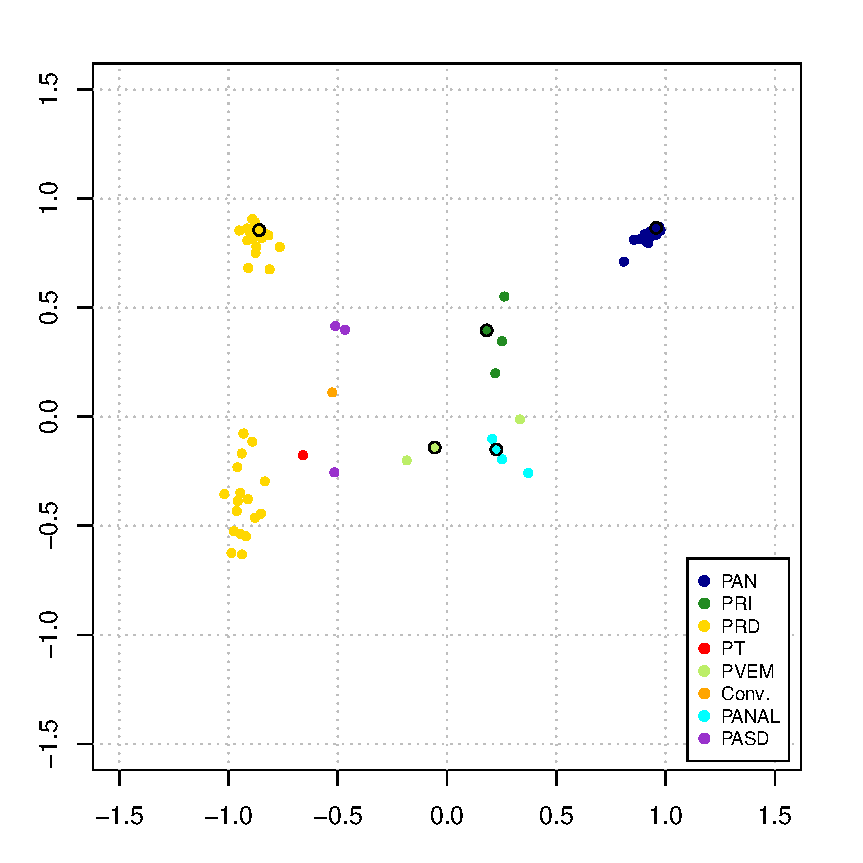
\includegraphics[width=8.25cm]{../graphs/static.pdf}
\end{tabular}
\end{center}

}

%%%%%%%%%%%%%%%%%%%%%%%%%%%%%%%%%%%%%%%%%%%%%%%%%%%%%%%%%%%%%%%%%%%%%%%%%%%%%%%%%%%%%%%%%%%%

\frame {                      % SLIDE

    \frametitle{Static estimation 2006--09}

\begin{center}
\begin{tabular}{c}
   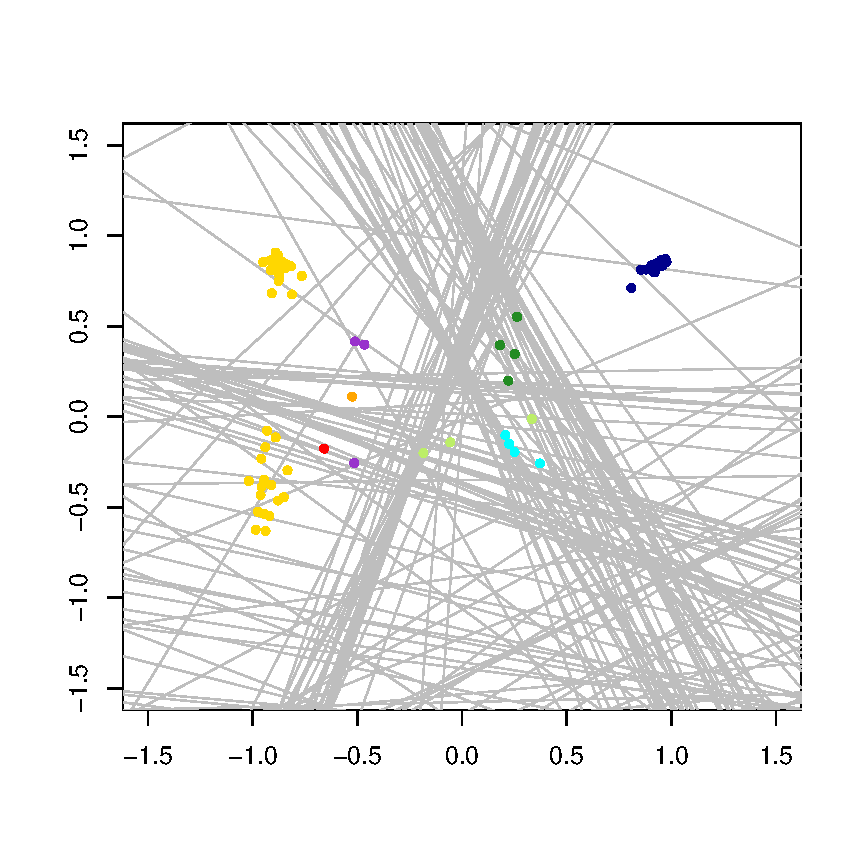
\includegraphics[width=9cm]{../graphs/staticcutlines.pdf}
\end{tabular}
\end{center}

}

%%%%%%%%%%%%%%%%%%%%%%%%%%%%%%%%%%%%%%%%%%%%%%%%%%%%%%%%%%%%%%%%%%%%%%%%%%%%%%%%%%%%%%%%%%%%

\frame {                      % SLIDE

    \frametitle{Dynamic model~~~~($t=1$)}

 \begin{columns}[c]

 \column{.85\textwidth}

\begin{center}
\begin{tabular}{c}
   \includegraphics[width=8cm]{../graphs/2006-3.pdf}
%   \includegraphics[width=8.25cm]{d:/01/data/rollcall/aldf/graphs/2006-3.pdf}
\end{tabular}
\end{center}

 \column{.15\textwidth}

\begin{tiny}
\begin{tabular}{ccc}
    2006 & \begin{tikzpicture} \draw[->,red,thick] (0,0) -- (.2,0); \end{tikzpicture} & \alert{\textbf{3}} \\
    2007 & \begin{tikzpicture} \draw (0,0) -- (.2,0); \end{tikzpicture} & 1 \\
         & \begin{tikzpicture} \draw (0,0) -- (.2,0); \end{tikzpicture} & 2 \\
         & \begin{tikzpicture} \draw (0,0) -- (.2,0); \end{tikzpicture} & 3 \\
    2008 & \begin{tikzpicture} \draw (0,0) -- (.2,0); \end{tikzpicture} & 1 \\
         & \begin{tikzpicture} \draw (0,0) -- (.2,0); \end{tikzpicture} & 2 \\
         & \begin{tikzpicture} \draw (0,0) -- (.2,0); \end{tikzpicture} & 3 \\
    2009 & \begin{tikzpicture} \draw (0,0) -- (.2,0); \end{tikzpicture} & 1 \\
\end{tabular}
\end{tiny}

\end{columns}


}

%%%%%%%%%%%%%%%%%%%%%%%%%%%%%%%%%%%%%%%%%%%%%%%%%%%%%%%%%%%%%%%%%%%%%%%%%%%%%%%%%%%%%%%%%%%%

\frame {                      % SLIDE

    \frametitle{Dynamic model~~~~($t=2$)}

 \begin{columns}[c]

 \column{.85\textwidth}

\begin{center}
\begin{tabular}{c}
   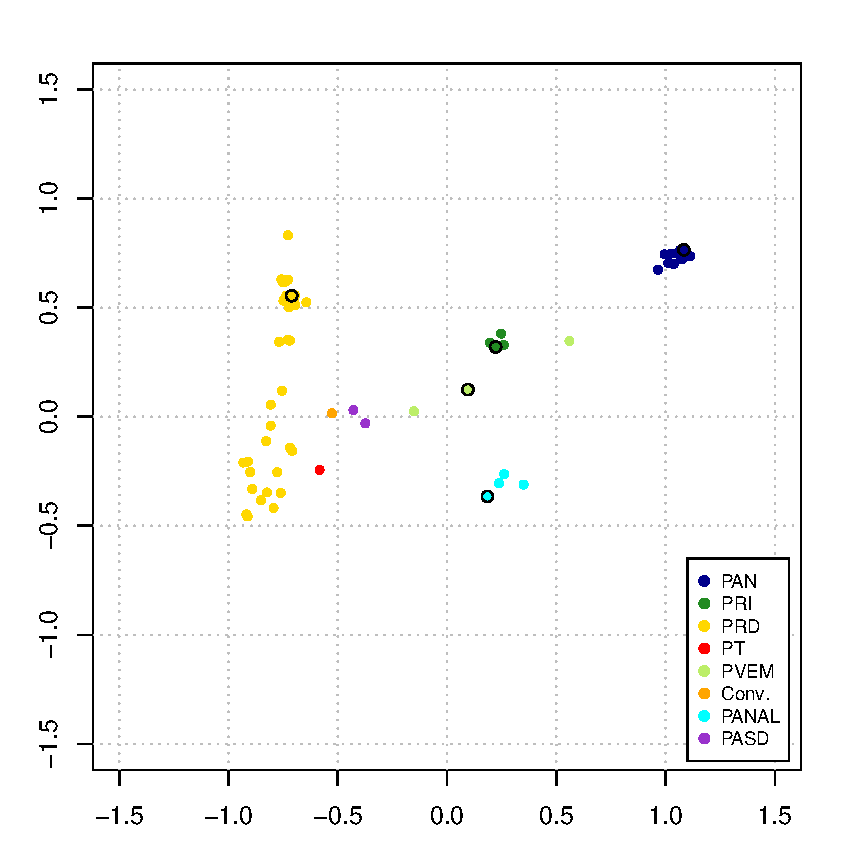
\includegraphics[width=8cm]{../graphs/2007-1.pdf}
%   \includegraphics[width=8.25cm]{d:/01/data/rollcall/aldf/graphs/2006-3.pdf}
\end{tabular}
\end{center}

 \column{.15\textwidth}

\begin{tiny}
\begin{tabular}{ccc}
    2006 & \begin{tikzpicture} \draw (0,0) -- (.2,0); \end{tikzpicture} & 3 \\
    2007 & \begin{tikzpicture} \draw[->,red,thick] (0,0) -- (.2,0); \end{tikzpicture} & \alert{\textbf{1}} \\
         & \begin{tikzpicture} \draw (0,0) -- (.2,0); \end{tikzpicture} & 2 \\
         & \begin{tikzpicture} \draw (0,0) -- (.2,0); \end{tikzpicture} & 3 \\
    2008 & \begin{tikzpicture} \draw (0,0) -- (.2,0); \end{tikzpicture} & 1 \\
         & \begin{tikzpicture} \draw (0,0) -- (.2,0); \end{tikzpicture} & 2 \\
         & \begin{tikzpicture} \draw (0,0) -- (.2,0); \end{tikzpicture} & 3 \\
    2009 & \begin{tikzpicture} \draw (0,0) -- (.2,0); \end{tikzpicture} & 1 \\
\end{tabular}
\end{tiny}

\end{columns}


}

%%%%%%%%%%%%%%%%%%%%%%%%%%%%%%%%%%%%%%%%%%%%%%%%%%%%%%%%%%%%%%%%%%%%%%%%%%%%%%%%%%%%%%%%%%%%

\frame {                      % SLIDE

    \frametitle{Dynamic model~~~~($t=3$)}

 \begin{columns}[c]

 \column{.85\textwidth}

\begin{center}
\begin{tabular}{c}
   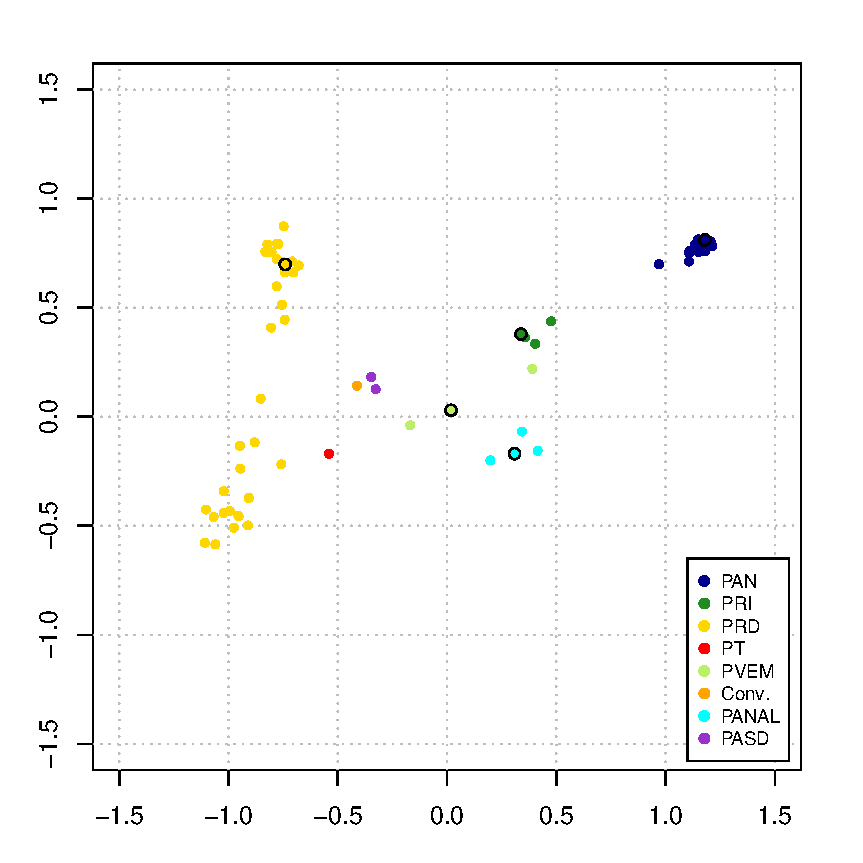
\includegraphics[width=8cm]{../graphs/2007-2.pdf}
%   \includegraphics[width=8.25cm]{d:/01/data/rollcall/aldf/graphs/2006-3.pdf}
\end{tabular}
\end{center}

 \column{.15\textwidth}

\begin{tiny}
\begin{tabular}{ccc}
    2006 & \begin{tikzpicture} \draw (0,0) -- (.2,0); \end{tikzpicture} & 3 \\
    2007 & \begin{tikzpicture} \draw (0,0) -- (.2,0); \end{tikzpicture} & 1 \\
         & \begin{tikzpicture} \draw[->,red,thick] (0,0) -- (.2,0); \end{tikzpicture} & \alert{\textbf{2}} \\
         & \begin{tikzpicture} \draw (0,0) -- (.2,0); \end{tikzpicture} & 3 \\
    2008 & \begin{tikzpicture} \draw (0,0) -- (.2,0); \end{tikzpicture} & 1 \\
         & \begin{tikzpicture} \draw (0,0) -- (.2,0); \end{tikzpicture} & 2 \\
         & \begin{tikzpicture} \draw (0,0) -- (.2,0); \end{tikzpicture} & 3 \\
    2009 & \begin{tikzpicture} \draw (0,0) -- (.2,0); \end{tikzpicture} & 1 \\
\end{tabular}
\end{tiny}

\end{columns}


}

%%%%%%%%%%%%%%%%%%%%%%%%%%%%%%%%%%%%%%%%%%%%%%%%%%%%%%%%%%%%%%%%%%%%%%%%%%%%%%%%%%%%%%%%%%%%

\frame {                      % SLIDE

    \frametitle{Dynamic model~~~~($t=4$)}

 \begin{columns}[c]

 \column{.85\textwidth}

\begin{center}
\begin{tabular}{c}
   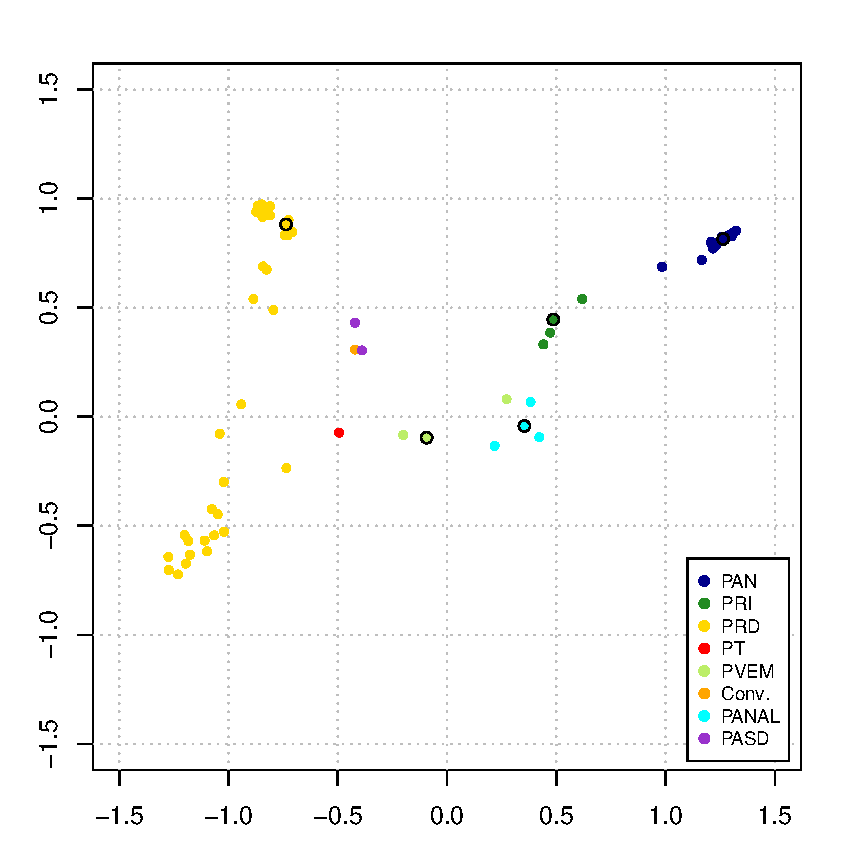
\includegraphics[width=8cm]{../graphs/2007-3.pdf}
%   \includegraphics[width=8.25cm]{d:/01/data/rollcall/aldf/graphs/2006-3.pdf}
\end{tabular}
\end{center}

 \column{.15\textwidth}

\begin{tiny}
\begin{tabular}{ccc}
    2006 & \begin{tikzpicture} \draw (0,0) -- (.2,0); \end{tikzpicture} & 3 \\
    2007 & \begin{tikzpicture} \draw (0,0) -- (.2,0); \end{tikzpicture} & 1 \\
         & \begin{tikzpicture} \draw (0,0) -- (.2,0); \end{tikzpicture} & 2 \\
         & \begin{tikzpicture} \draw[->,red,thick] (0,0) -- (.2,0); \end{tikzpicture} & \alert{\textbf{3}} \\
    2008 & \begin{tikzpicture} \draw (0,0) -- (.2,0); \end{tikzpicture} & 1 \\
         & \begin{tikzpicture} \draw (0,0) -- (.2,0); \end{tikzpicture} & 2 \\
         & \begin{tikzpicture} \draw (0,0) -- (.2,0); \end{tikzpicture} & 3 \\
    2009 & \begin{tikzpicture} \draw (0,0) -- (.2,0); \end{tikzpicture} & 1 \\
\end{tabular}
\end{tiny}

\end{columns}


}

%%%%%%%%%%%%%%%%%%%%%%%%%%%%%%%%%%%%%%%%%%%%%%%%%%%%%%%%%%%%%%%%%%%%%%%%%%%%%%%%%%%%%%%%%%%%

\frame {                      % SLIDE

    \frametitle{Dynamic model~~~~($t=5$)}

 \begin{columns}[c]

 \column{.85\textwidth}

\begin{center}
\begin{tabular}{c}
   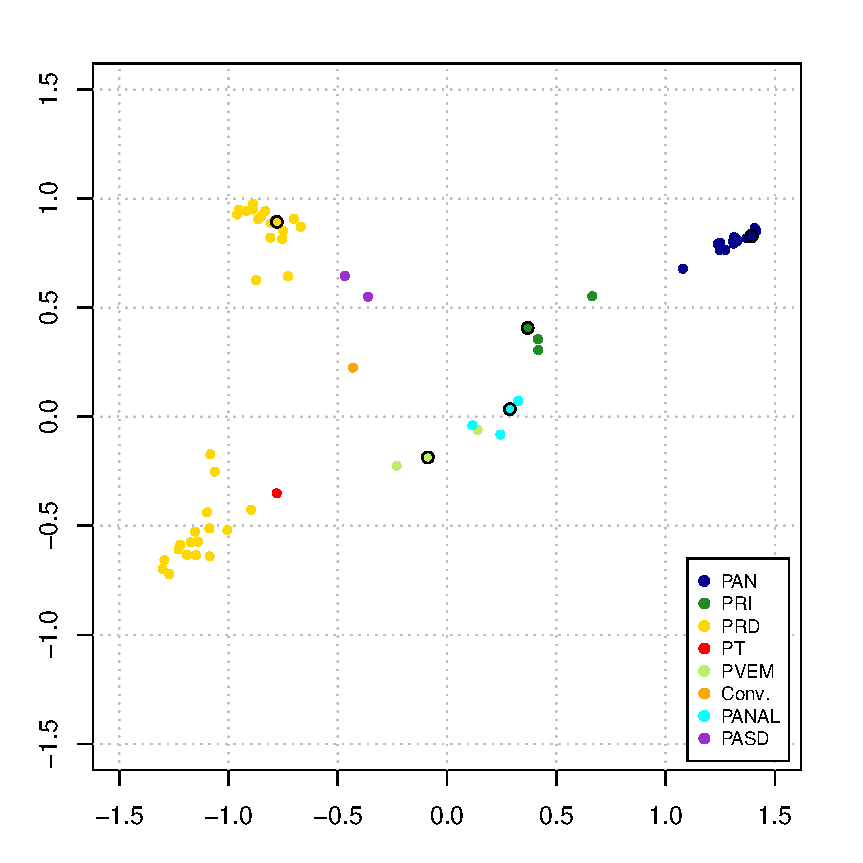
\includegraphics[width=8cm]{../graphs/2008-1.pdf}
%   \includegraphics[width=8.25cm]{d:/01/data/rollcall/aldf/graphs/2006-3.pdf}
\end{tabular}
\end{center}

 \column{.15\textwidth}

\begin{tiny}
\begin{tabular}{ccc}
    2006 & \begin{tikzpicture} \draw (0,0) -- (.2,0); \end{tikzpicture} & 3 \\
    2007 & \begin{tikzpicture} \draw (0,0) -- (.2,0); \end{tikzpicture} & 1 \\
         & \begin{tikzpicture} \draw (0,0) -- (.2,0); \end{tikzpicture} & 2 \\
         & \begin{tikzpicture} \draw (0,0) -- (.2,0); \end{tikzpicture} & 3 \\
    2008 & \begin{tikzpicture} \draw[->,red,thick] (0,0) -- (.2,0); \end{tikzpicture} & \alert{\textbf{1}} \\
         & \begin{tikzpicture} \draw (0,0) -- (.2,0); \end{tikzpicture} & 2 \\
         & \begin{tikzpicture} \draw (0,0) -- (.2,0); \end{tikzpicture} & 3 \\
    2009 & \begin{tikzpicture} \draw (0,0) -- (.2,0); \end{tikzpicture} & 1 \\
\end{tabular}
\end{tiny}

\end{columns}


}

%%%%%%%%%%%%%%%%%%%%%%%%%%%%%%%%%%%%%%%%%%%%%%%%%%%%%%%%%%%%%%%%%%%%%%%%%%%%%%%%%%%%%%%%%%%%

\frame {                      % SLIDE

    \frametitle{Dynamic model~~~~($t=6$)}

 \begin{columns}[c]

 \column{.85\textwidth}

\begin{center}
\begin{tabular}{c}
   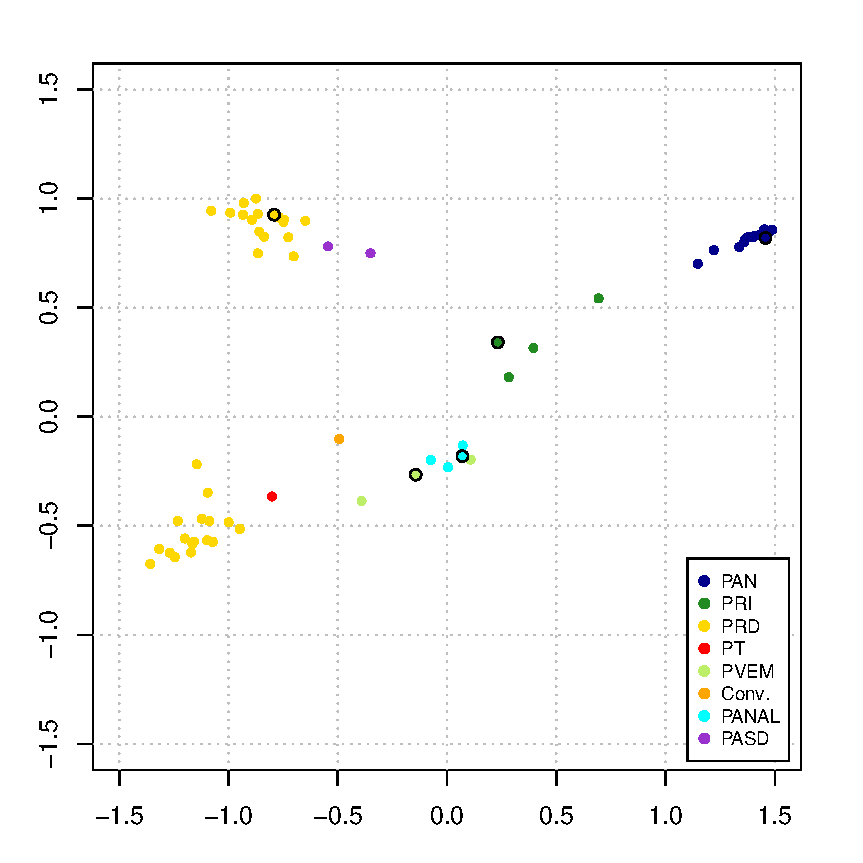
\includegraphics[width=8cm]{../graphs/2008-2.pdf}
%   \includegraphics[width=8.25cm]{d:/01/data/rollcall/aldf/graphs/2006-3.pdf}
\end{tabular}
\end{center}

 \column{.15\textwidth}

\begin{tiny}
\begin{tabular}{ccc}
    2006 & \begin{tikzpicture} \draw (0,0) -- (.2,0); \end{tikzpicture} & 3 \\
    2007 & \begin{tikzpicture} \draw (0,0) -- (.2,0); \end{tikzpicture} & 1 \\
         & \begin{tikzpicture} \draw (0,0) -- (.2,0); \end{tikzpicture} & 2 \\
         & \begin{tikzpicture} \draw (0,0) -- (.2,0); \end{tikzpicture} & 3 \\
    2008 & \begin{tikzpicture} \draw (0,0) -- (.2,0); \end{tikzpicture} & 1 \\
         & \begin{tikzpicture} \draw[->,red,thick] (0,0) -- (.2,0); \end{tikzpicture} & \alert{\textbf{2}} \\
         & \begin{tikzpicture} \draw (0,0) -- (.2,0); \end{tikzpicture} & 3 \\
    2009 & \begin{tikzpicture} \draw (0,0) -- (.2,0); \end{tikzpicture} & 1 \\
\end{tabular}
\end{tiny}

\end{columns}


}

%%%%%%%%%%%%%%%%%%%%%%%%%%%%%%%%%%%%%%%%%%%%%%%%%%%%%%%%%%%%%%%%%%%%%%%%%%%%%%%%%%%%%%%%%%%%

\frame {                      % SLIDE

    \frametitle{Dynamic model~~~~($t=7$)}

 \begin{columns}[c]

 \column{.85\textwidth}

\begin{center}
\begin{tabular}{c}
   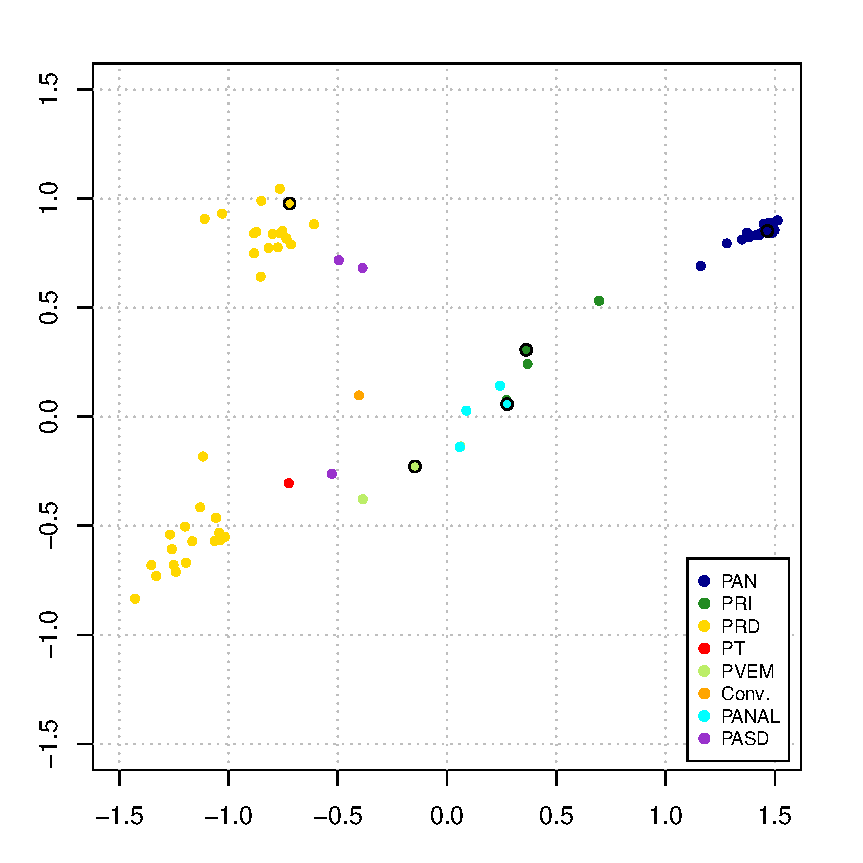
\includegraphics[width=8cm]{../graphs/2008-3.pdf}
%   \includegraphics[width=8.25cm]{d:/01/data/rollcall/aldf/graphs/2006-3.pdf}
\end{tabular}
\end{center}

 \column{.15\textwidth}

\begin{tiny}
\begin{tabular}{ccc}
    2006 & \begin{tikzpicture} \draw (0,0) -- (.2,0); \end{tikzpicture} & 3 \\
    2007 & \begin{tikzpicture} \draw (0,0) -- (.2,0); \end{tikzpicture} & 1 \\
         & \begin{tikzpicture} \draw (0,0) -- (.2,0); \end{tikzpicture} & 2 \\
         & \begin{tikzpicture} \draw (0,0) -- (.2,0); \end{tikzpicture} & 3 \\
    2008 & \begin{tikzpicture} \draw (0,0) -- (.2,0); \end{tikzpicture} & 1 \\
         & \begin{tikzpicture} \draw (0,0) -- (.2,0); \end{tikzpicture} & 2 \\
         & \begin{tikzpicture} \draw[->,red,thick] (0,0) -- (.2,0); \end{tikzpicture} & \alert{\textbf{3}} \\
    2009 & \begin{tikzpicture} \draw (0,0) -- (.2,0); \end{tikzpicture} & 1 \\
\end{tabular}
\end{tiny}

\end{columns}


}

%%%%%%%%%%%%%%%%%%%%%%%%%%%%%%%%%%%%%%%%%%%%%%%%%%%%%%%%%%%%%%%%%%%%%%%%%%%%%%%%%%%%%%%%%%%%

\frame {                      % SLIDE

    \frametitle{Dynamic model~~~~($t=8$)}

 \begin{columns}[c]

 \column{.85\textwidth}

\begin{center}
\begin{tabular}{c}
   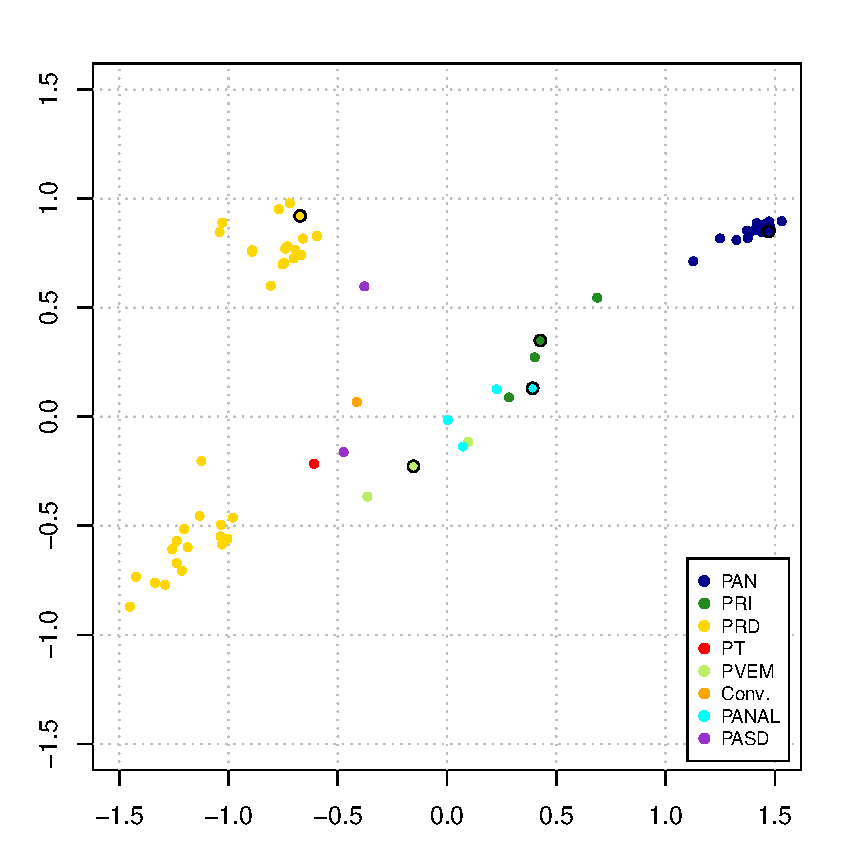
\includegraphics[width=8cm]{../graphs/2009-1.pdf}
%   \includegraphics[width=8.25cm]{d:/01/data/rollcall/aldf/graphs/2006-3.pdf}
\end{tabular}
\end{center}

 \column{.15\textwidth}

\begin{tiny}
\begin{tabular}{ccc}
    2006 & \begin{tikzpicture} \draw (0,0) -- (.2,0); \end{tikzpicture} & 3 \\
    2007 & \begin{tikzpicture} \draw (0,0) -- (.2,0); \end{tikzpicture} & 1 \\
         & \begin{tikzpicture} \draw (0,0) -- (.2,0); \end{tikzpicture} & 2 \\
         & \begin{tikzpicture} \draw (0,0) -- (.2,0); \end{tikzpicture} & 3 \\
    2008 & \begin{tikzpicture} \draw (0,0) -- (.2,0); \end{tikzpicture} & 1 \\
         & \begin{tikzpicture} \draw (0,0) -- (.2,0); \end{tikzpicture} & 2 \\
         & \begin{tikzpicture} \draw (0,0) -- (.2,0); \end{tikzpicture} & 3 \\
    2009 & \begin{tikzpicture} \draw[->,red,thick] (0,0) -- (.2,0); \end{tikzpicture} & \alert{\textbf{1}} \\
\end{tabular}
\end{tiny}

\end{columns}


}

%%%%%%%%%%%%%%%%%%%%%%%%%%%%%%%%%%%%%%%%%%%%%%%%%%%%%%%%%%%%%%%%%%%%%%%%%%%%%%%%%%%%%%%%%%%%%%%%

\frame {                      % SLIDE

    \frametitle{Findings and next steps}

Preliminary analysis reveals that:

\begin{enumerate}

\item Majority united in left--right axis, \\ but split consistently over ``confirmations''

\item $4^{th}$ legislature exceptional? Routine?

\item 2006 fiasco may explain

\item Verify studying other legislatures

\item Check Bonica's work

\end{enumerate}

\pause

\bigskip

\center{\textbf{\Large{Thank you!}}}

}

%%%%%%%%%%%%%%%%%%%%%%%%%%%%%%%%%%%%%%%%%%%%%%%%%%%%%%%%%%%%%%%%%%%%%%%%%%%%%%%%%%%%%%%%%%%%

\frame {                      % SLIDE

    \frametitle{Bi-dimensionality}

\begin{figure}
\begin{center}
   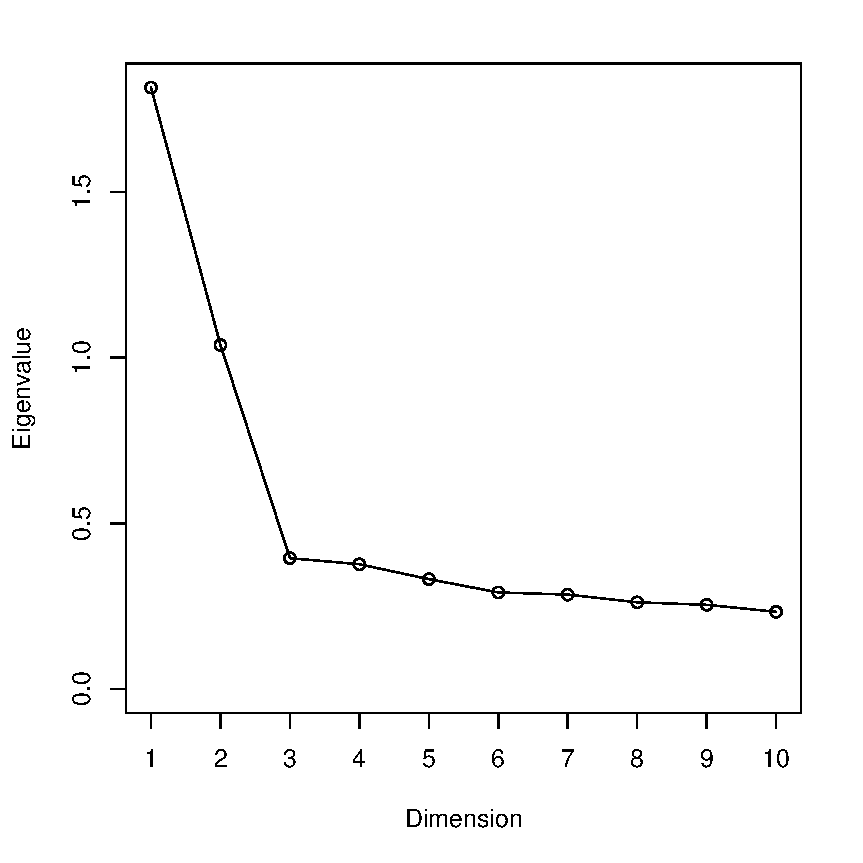
\includegraphics[width=6cm]{../graphs/eigenvalues.pdf} \\
 \caption{\footnotesize{Eigenvalues of the double-centered agreement score matrix for 4th legislature drop fairly smoothly from the third value onwards, an indication that the data are most likely two-dimensional. Abstentions and absences coded as nays for this computation.}}
\end{center}
\end{figure}

}

\end{document}
